\documentclass[conference]{IEEEtran}
\IEEEoverridecommandlockouts
% The preceding line is only needed to identify funding in the first footnote. If that is unneeded, please comment it out.
\usepackage{cite}
\usepackage{amsmath,amssymb,amsfonts}
\usepackage{algorithmic}
\usepackage{graphicx}
\usepackage{textcomp}
\usepackage{xcolor}
\def\BibTeX{{\rm B\kern-.05em{\sc i\kern-.025em b}\kern-.08em
    T\kern-.1667em\lower.7ex\hbox{E}\kern-.125emX}}
\begin{document}

\title{Experimental investigation of forced convective heat transfer in cylindrical pipe flow\\
%{\footnotesize \textsuperscript{*}Note: Sub-titles are not captured in Xplore and should not be used}
%\thanks{Identify applicable funding agency here. If none, delete this.}
}

\author{\IEEEauthorblockN{Yoshinori Hattori}
\IEEEauthorblockA{\textit{Shibaura Institute of Technology, Mechanical Engineering}\\
Tokyo, Japan \\
\textit{Graz University of Technology, Institute of Fluid Mechanics and Heat Transfer}\\
Graz, Austria \\
md18060@shibaura-it.ac.jp}}

\maketitle

%\begin{abstract}
%This document is a model and instructions for \LaTeX.
%This and the IEEEtran.cls file define the components of your paper [title, text, heads, etc.]. *CRITICAL: Do Not Use Symbols, Special Characters, Footnotes,
%or Math in Paper Title or Abstract.
%\end{abstract}

\begin{IEEEkeywords}
Forced convection, Nusselt number, Wall friction, transitional, Cylindrical pipe flow
\end{IEEEkeywords}

\section{Introduction}
In recent years, forced convective heat transfer in cylindrical pipe flow plays an important role in many technical cooling systems.
Nusselt number (Nu) is a dimensionless number which represents the ratio of convective (h) and conductive heat transfer (k), as expressed in Equation \eqref{Nu_number}.
\begin{equation}
Nu=\frac{h\cdot L}{k}\label{Nu_number}
\end{equation}
From general dimensional analysis, Nusselt number represents function of Reynolds number (Re) times Prandtl number (Pr) as Equation \eqref{Nu_dimensional}.
\begin{equation}
Nu=\alpha \cdot Re^{\pi_{\beta}}\cdot Pr^{\pi_{\gamma}}\label{Nu_dimensional}
\end{equation}
Here, factors $\alpha$, $\beta$ and $\gamma$ are constant values that depend on flow regime and are calculated from an experimental result.
Nusselt number is one of the most important numbers for forced convective heat transfer, and are calculated from Equation \eqref{Nu_number} and \eqref{Nu_dimensional}.

Many studies have pointed out that a heat transfer coefficient varies depending on the type of flow: laminar, transition and turbulent.
Gnienlinski\cite{Gnienlinski2010} showed a calculation method for the laminar heat transfer coefficient of two kinds of boundary conditions. (I) Constant wall temperature (UWT) and (I\hspace{-.1em}I) Constant heat flux (UHF).
Petukhvov and Kirillov\cite{Petukhov1958} showed calculation method for turbulent flows.
There has been very scarce experimental data of laminar-to-turbulent transitional region.
Bertsche et al,\cite{Bertsche2016} focused on reliable prediction of heat transfer coefficient for transitional flows.
In their study, Bertsche et al, showed experimental heat transfer coefficients for Reynolds number $500 < Re < 23000$ and Prandtl number $7 < Pr < 41$.

Much remains to be studied for providing experimental data except water and glycole as operation fluids.
In this study, I focused on forced convective heat transfer in flow of water and glycole in a cylindrical pipe.
A 50/50vol\% mixture of water and glycole, which is a typical liquid coolant in automotive applications was used as a operating fluid.
The experiment was carried out by considering a board range of Reynolds numbers, spanning from a laminar to fully turbulent flow.
Moreover, the measurement of wall friction coefficients were also performed in this study.
The experimental data were compared with other sources as well as computational results obtained from already existing numerical simulations (CFD) by Christphan \cite{Christphan2018}.



%\section{The phenomena}
%%Temperature variations for constantHeat flux
%\begin{figure}[htbp]
%  \centering
%  %\vspace{-3zh}
%  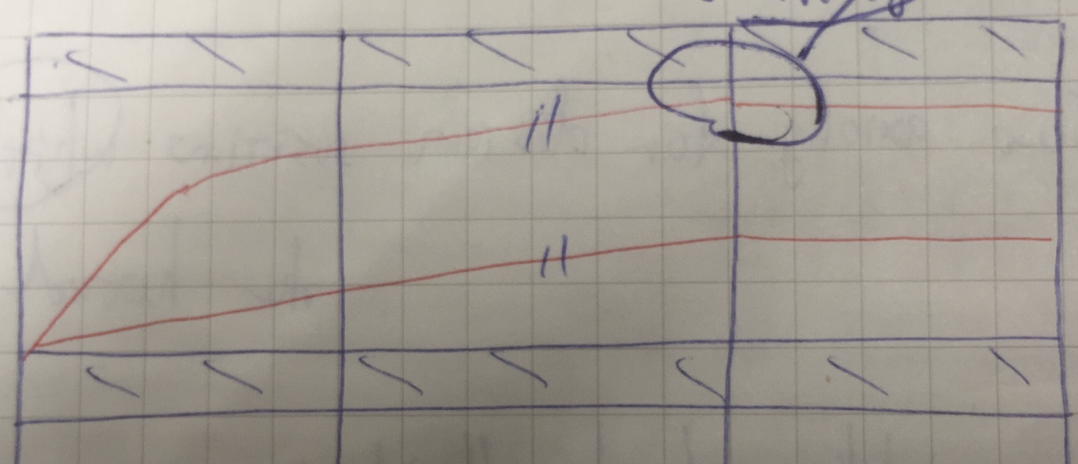
\includegraphics[width=0.47\textwidth,natwidth=610,natheight=642]{fig/temperature_variations_constant_heat_flux.png}
%  \caption{Temperature variations for constantHeat flux}
%  \label{temperature_variations_constant_heat_flux}
%\end{figure}
%
%%Heat transfer coefficient depend on x value
%Figure\label{heat_transfer_coefficient_depend_on_x_value} shows the local heat transfer coeeficient 
%\begin{figure}[htbp]
%  \centering
%  %\vspace{-3zh}
%  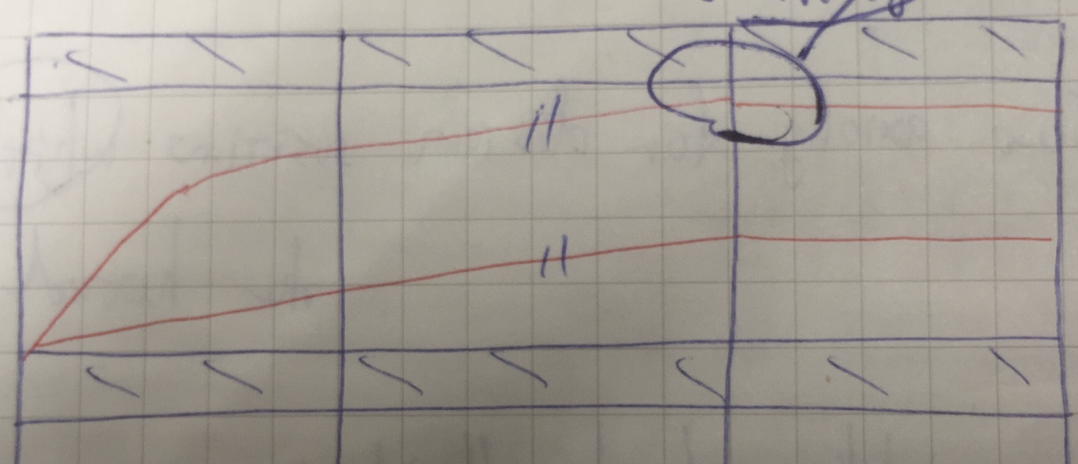
\includegraphics[width=0.47\textwidth,natwidth=610,natheight=642]{fig/temperature_variations_constant_heat_flux.png}
%  \caption{Heat transfer coefficient depend on x value}
%  \label{heat_transfer_coefficient_depend_on_x_value}
%\end{figure}
%There are two surface conditions arise in many engineering applications.
%One is constant surface heat flux and the other is constant surface temperature.
%In the fully developed flow of the tube, fluid constant porperties, the local heat coefficient is constant independent of x.

\section{Experimental setup}
%Experimental Setup
Figure. \ref{experimental_loop} shows experimental loop.
The experimental loop consists of heat exchanger, pump, coriolis mass flow rate, welder, reservoir, and test section basically.
Heat exchenger keep thermal stationary condition in flow pipe.
Mass flow rate is controlled by pump and baypass valve C which is located in a parallel.
The pipe is thermal isolated, surrounded with glass wool.\\

\begin{figure}[htbp]
\centering
\vspace{-4zh}
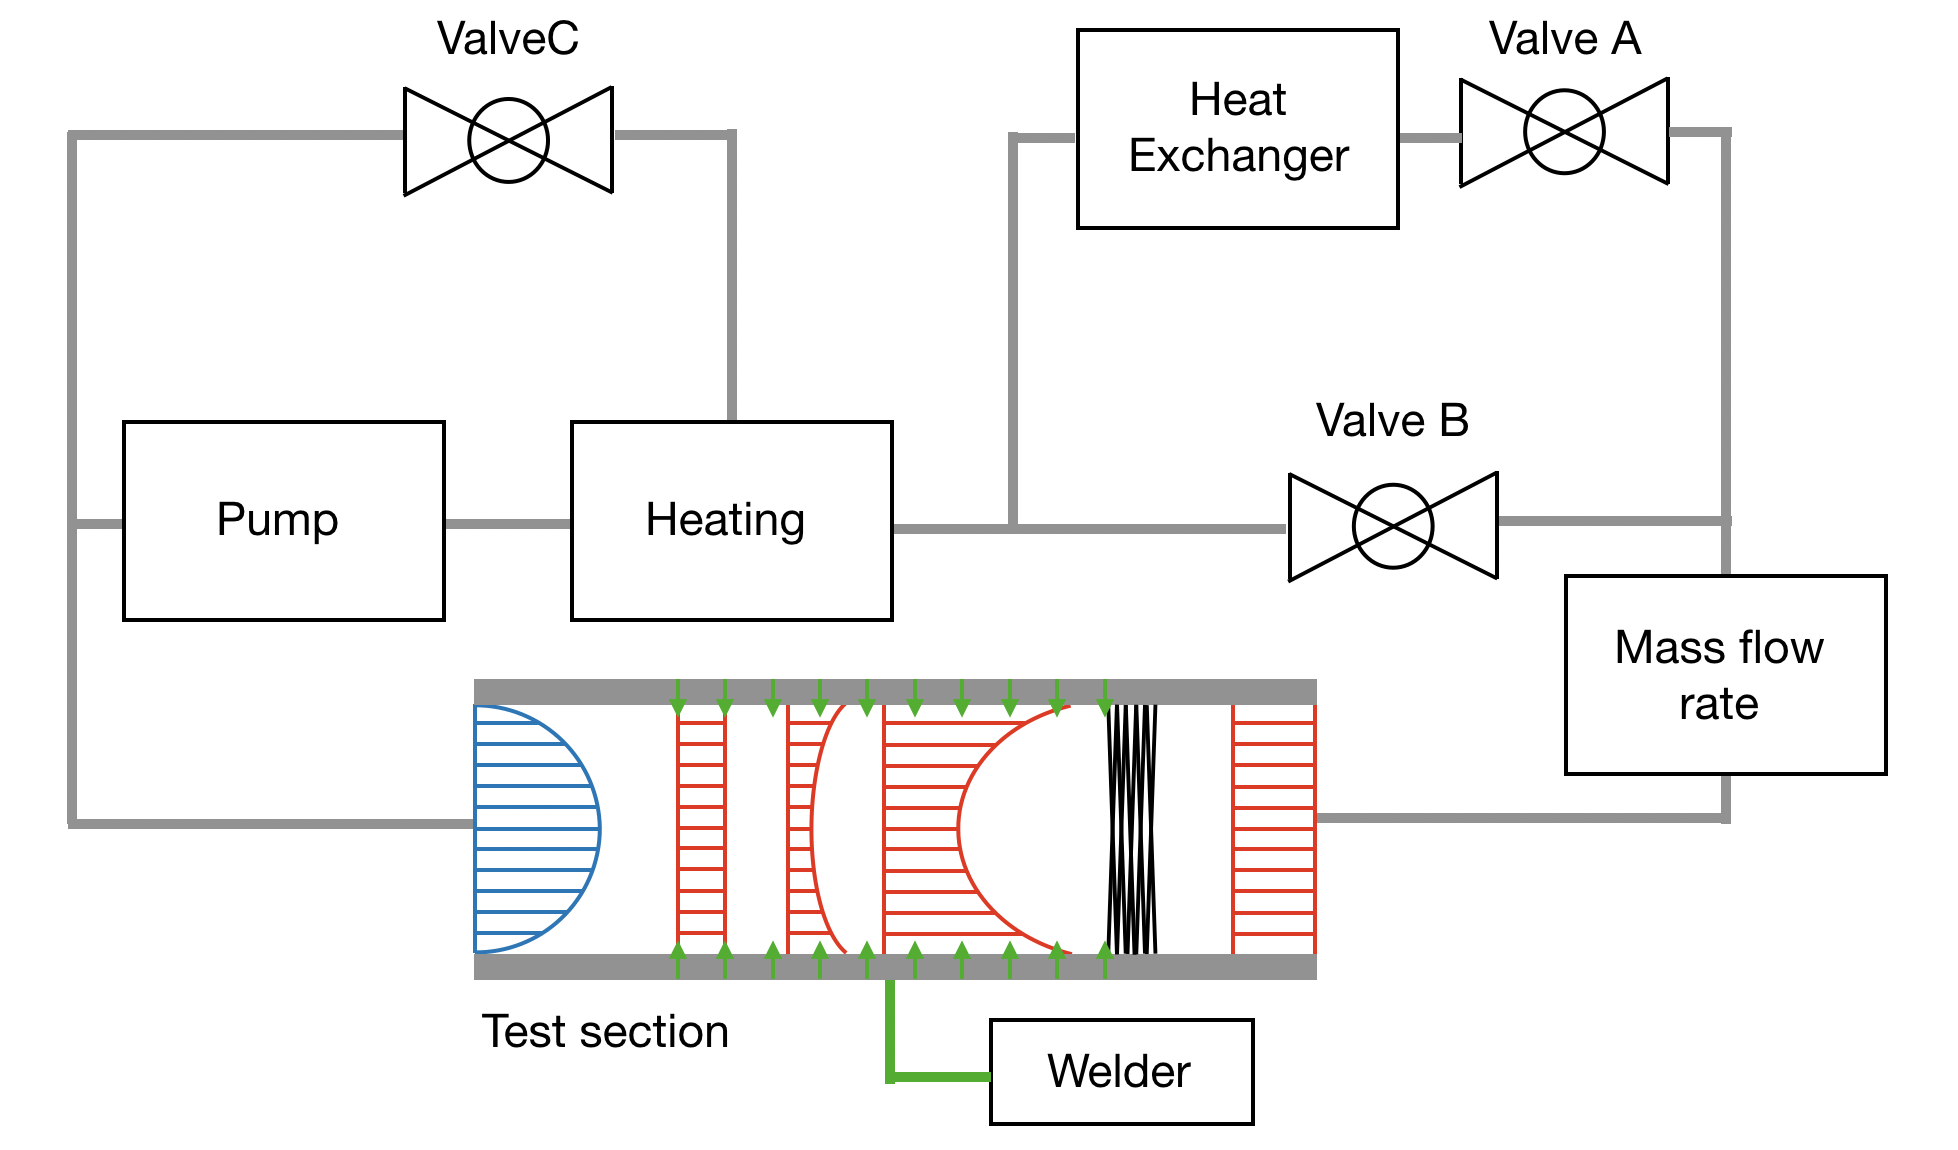
\includegraphics[width=0.47\textwidth,natwidth=920,natheight=700]{fig/experimental_loop.png}
\caption{Process flow diagram of the test facilities including test section.}
\label{experimental_loop}
\end{figure}

Figure. \ref{thermal_boundary_layer_development} shows velocity and thermal boundary layer development vary with horizontal axis in a test section.
Velocity and thermal profile are shown blue and red color, respectively.
The test section is made of stainless steel (1.4301) with an inner diameter di=12mm and outer diameter do= 15mm.
Highly accurate resistance thermall probes (PT-100) are used to find out the inlet and outlet bulk temperature (Tib , Tob) and wall temperature Tw.
Moreover, thermocouple 'Type-K' are used to take temperature gradient in flow direction.
\newpage
The test section consist of entrance, heated and thermal equalized part.
\begin{enumerate}
  \item Entrance part\\
  The first part of test section is 1.2 [m] length entrance part which is sufficiently long to ensure dynamically developed flow condition at the exist.
  The bulk temperature (Tb0) at this section were measured by PT-100.
  \item Heated part\\
  The second part of test section is 2 [m] length heated part which is sufficiently long to ensure thermaly fully developed flow condition at the exist.
  The tube wall were heated electrically by welder which provide high current and low voltage to keep the uniform heat flux condition in a inner pipe flow. 
  Convective heat transfer is independent with horizontal axis in fully developed flow, constant heat flux condition.
  The wall temperature (Tw) at the exist of this section were measured by PT-100.
  \item Thermal equalized part\\
  The third part of test section is thermall equalized part which is including static mixture. Static mixture forms turbulent and vortex. Then, the thermal profile of heated exist mix together. At the end, the bulk temperature(Tb1) are measured.
\end{enumerate}


\begin{figure}[htbp]
  \centering
  %\vspace{-3zh}
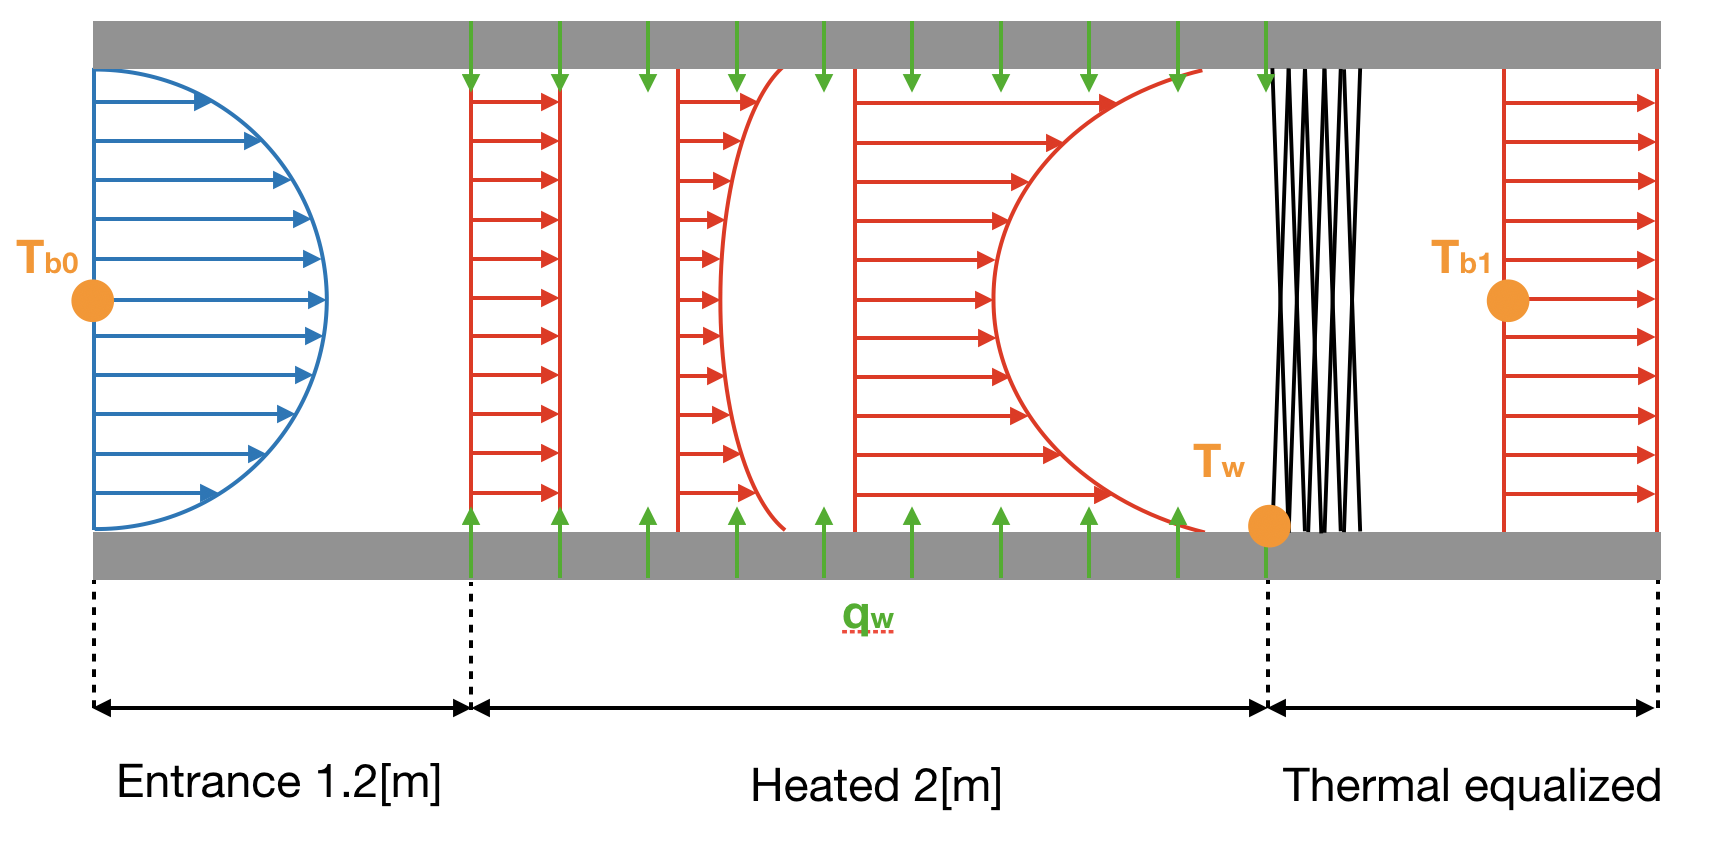
\includegraphics[width=0.47\textwidth,natwidth=850,natheight=450]{fig/thermal_boundary_layer_development.png}
  \caption{Velocity (blue) and thermal (red) boundary layer development vary with horizontal axis in a test section.}
  \label{thermal_boundary_layer_development}
\end{figure}

\section{Calucuration Flow}
Material properties are all temperature-dependent function.
At first, material properties varies with temperature were taken.
Next, I move to experimental facilities and measured temperature differences, pressure differences and mass flow rates.
Finaly, Nusselt, Prandtl, Reynolds numbers and friction coefficients were calcurated by post-proccesing, LabView and MATLAB. 

%\section{Correlations}
%Skinf friction coefficient for laminar flow is descrived following equation.
%\begin{equation}
%C_{f,lam}=\frac{16}{Re_{b}}
%\end{equation}
%Konakov\cite{Konakov1954} showed skin friction coefficient for turbulent flow.
%\begin{equation}
%C_{f,turb}=0.25(1.8log(Re_{b})-1.5)^{-2}
%\end{equation}
%Note that these skin friction coefficient just suitable for no-heating condition, constant fluid properties.
%In this thesis, we provide heat to the pipe.
%Therefore, the fluid properties change depend on the temperature.
%
%From general dimensional analysis, Nusselt number represents function of Reynolds number (Re) times Prandtl number (Pr) as following equation.
%\begin{equation}
%Nu=\alpha \cdot Re^{\pi_{\beta}}\cdot Pr^{\pi_{\gamma}}\label{Nu_dimensional}
%\end{equation}
%Here, factors $\alpha$, $\beta$ and $\gamma$ are constant value depend on flow regime and calcurated from numerical experimental results.
%Gunienski\cite{Gnienlinski2010} showed correlations for each flow regime laminar and turbulent, respectively.
%Gunienski\cite{Gnienlinski2010} showed calculation method for laminar flow.
%\begin{equation}
%Nu_{lam}=(3.66^{3}+0.7^{3}+(1.615(Re_{b}Pr_{b}\frac{d_{i}}{L})^{1/3})^{3})^{1/3}\label{Nu_laminar}
%\end{equation}
%%The range 0.1<<Pr_{b}<<1000, 10^{4}<<Re_{b}<<10^{6}.
%Gunienski\cite{Gnienlinski2010} showed calculation method for turbulent flow.
%\begin{equation}
%Nu_{turb}=\frac{\frac{C_{f}}{2Re\cdot Pr_{b}}}{1+12.7 \sqrt{\frac{C_{f}}{2}}(Pr_{b}^{2/3}-1)}\cdot (\frac{Pr_{b}}{Pr_{w}})^{0.11}
%%Nu_{turb}=\frac{\frac{C_{f}}{2\cdot Re\cdot Pr_{b}}{(1+12.7\frac{C_{f}}{2}}\cdot (Pr^{\frac{2}{3}}-1)}\cdot(1+(\frac{d_{h}}{l})^{\frac{2}{3}})\label{Nu_turblent}
%\end{equation}
%The range is
%\begin{equation}
%0.1<<Pr_{b}<<1000, 10^{4}<<Re_{b}<<10^{6}.
%\end{equation}
%He presented transitional flow as a liner interpolation between turbulent and laminar flow.
%(See ''science problems and interesting issue'' section No.12.)
%\begin{equation}
%Nu_{m}=(1-r)Nu_{m,lam}+rNu_{m,turb}
%\label{Nu_m}
%\end{equation}
%\begin{equation}
%r=\frac{Re_{b}-2300}{10^{4}-2300}
%\end{equation}
%\\

\section{Results and Discussion}
The Density rho, heat conductivity k, specific heat transfer Cp, kinetic viscosity nu, dynamic viscosity mu, Pradtl number Pr are all varies with temperature.
It is difficult to keep high Pramdlt number and transitional Reynolds number.
For example, as enhance cooling, temperature decrease,
statics viscosity increase.
As a result, Pr increase and Re decrease.
An Experimental data and correlations were compared.
In correlations, the Prandtl number was assumed to be constant.
However, the experimental Prandtl number is not constant because the fluid properties vary with temperature.
The aim is to set Prandlt number level and vary the Reynolds number.
The avaraged Prandlt numbers were taken to plot Nusselt and Reynolds number. \\
Figure. \ref{result} shows heat transfer coefficients for 500 $<$ Re $<$ 4000 for Pr = 26, which shows good agreement with calcuration method showed by Gnienski of each flow regime, laminar, transitional and turbulent.\\
200 experimental results (500 $<$ Re $<$ 4000 and 10 $<$ Pr $<$ 30) has been compared with calcurations method for predictiong the laminar, transitional and turbulent heat transfer coefficiets.

\begin{figure}[htbp]
  \centering
  \vspace{4zh}
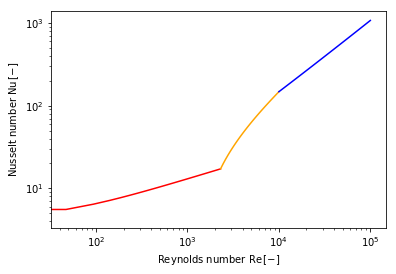
\includegraphics[width=0.47\textwidth,natwidth=400,natheight=200]{fig/result.png}
  \caption{Dimensionless heat transfer coefficients compared to literature data for Pr = 26. The red, yellow and blue lines are Gnielinski correlations for laminar, transitional and turbulent, respectively.}
  \label{result}
\end{figure}


%\section{Measurement uncertainty}
%The uncertainty of measurement was analyzed by using ``Guide to the Expression of Uncertainty in Measurement``(GUM).
%\\

\section{Conclusion}
Forced convective heat transfer in cylindrical pipe flow has been investigated experimentally.
Not so many data were available for transitional regime and high Prandtl number.
Therefore, in this study, 200 experimental results (500 $<$ Re $<$ 4000, 10 $<$ Pr $<$ 30) has been checked with calcuration method showed by Gnielinski\cite{Gnienlinski2010} and it showed good agreement.

\section{Acknowledgement}
I would like to thank my thesis advisors Prof. Helfried
Steiner and Prof. Guenter Brenn of the Institute of Fluid Mechanics and Heat Transfer at Graz University of Technology.
I am also grateful to Dr. Shirai of Mechanical Engineering
department at Shibaura Institute of Technology. I am extremely
thankful and indebted to him for sharing his experiments. I
would also like to thank Dr. Tange allowed my studying in out of Shibaura Institute of Technology.
\\


\begin{thebibliography}{00}
 \bibitem{Frank} Frank P. Incropera, David P. DeWitt, ``Fundamentals of Heat and Mass Transfer,'' 4th edition., WILEY, 1996.
 \bibitem{Gnienlinski2010} V. Gnienlinski, ``Heat Transfer in Laminar Flow,'' VDI Heat Atlas, second ed., Springer Verlag, 2010 (Chapter Ga 1-7), Section 3.
 \bibitem{Petukhov1958} B.S. Petukhov, V.V. kirillov, Teploenergetika 4 (1958) 91-98.
 \bibitem{Bertsche2016} Dirk Bertsche, Paul Knipper, Thomas Wetzel, ``Experimental investigation on heat transfer in laminar, transitional and turbulent circular pipe flow,'' International Journal of Heat Transfer, 95 (2016) 1008-1018.
\bibitem{Christphan2018} Christphan, ``Title of paper if known,'' unpublished, 2018.
\bibitem{Konakov1954} Konakov, ``Eine neue Formel fr den Reibungskoezienten glatter Rohre,'' Bericht der Akademie der Wissenschaften der UDSSR 51.7, 503-506.
% \bibitem{b5} R. Nicole, ``Title of paper with only first word capitalized,'' J. Name Stand. Abbrev., in press.
% \bibitem{b6} Y. Yorozu, M. Hirano, K. Oka, and Y. Tagawa, ``Electron spectroscopy studies on magneto-optical media and plastic substrate interface,'' IEEE Transl. J. Magn. Japan, vol. 2, pp. 740--741, August 1987 [Digests 9th Annual Conf. Magnetics Japan, p. 301, 1982].
% \bibitem{b7} M. Young, The Technical Writer's Handbook. Mill Valley, CA: University Science, 1989.

%\bibliography{junsrt}
%\bibliography{project_forced_convective@Graz.bib}

\end{thebibliography}
%\vspace{12pt}
%\color{red}
%IEEE conference templates contain guidance text for composing and formatting conference papers. Please ensure that all template text is removed from your conference paper prior to submission to the conference. Failure to remove the template text from your paper may result in your paper not being published.

\end{document}
